\section{Introducción}

\begin{slide}
  \begin{block}{\textbf{Orígenes de la navegación por satélite}}
    \begin{minipage}[b]{0.7\linewidth}
      \begin{itemize}
        \item Transit
        \begin{itemize}
          \item[$\rightarrow$] 60's
          \item[$\rightarrow$] Ejército EEUU
        \end{itemize}
        \item<2> Acura Legend
        \begin{itemize}
          \item[$\rightarrow$] 80's
          \item[$\rightarrow$] Honda
        \end{itemize}
      \end{itemize}
    \end{minipage}
    \begin{minipage}[b]{0.2\linewidth}
      \begin{figure}
        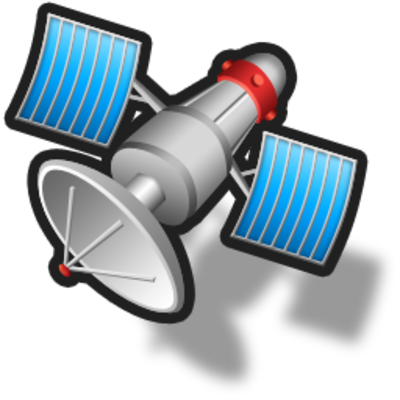
\includegraphics[height=0.4\textheight]{img/satellite.png}
      \end{figure}
    \end{minipage}
  \end{block}
\end{slide}

\begin{slide}
  \begin{block}{\textbf{Actualidad de la navegación por satélite}}
  \begin{center}
    \begin{minipage}[b]{0.3\linewidth}
      \begin{center}
        \begin{figure}
          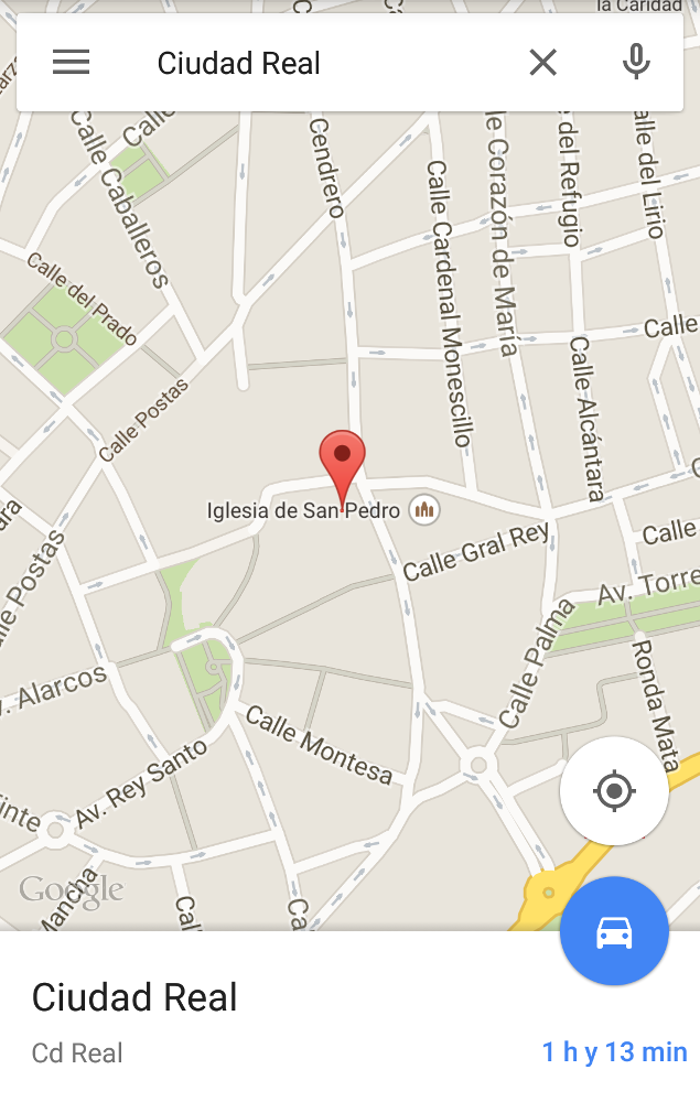
\includegraphics[height=0.6\textheight]{img/googlemaps.png}
        \end{figure}
        Google Maps
      \end{center}
    \end{minipage}
    \begin{minipage}[b]{0.3\linewidth}
      \begin{center}
        \begin{figure}
          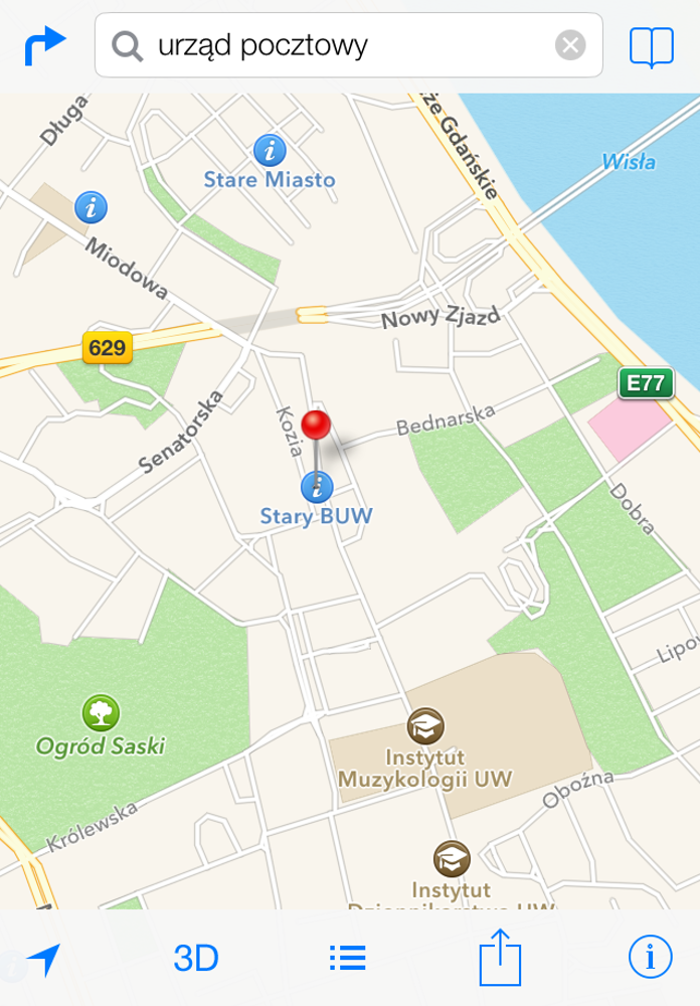
\includegraphics[height=0.6\textheight]{img/iosmaps.png}
        \end{figure}
        iOS Maps
      \end{center}
    \end{minipage}
    \begin{minipage}[b]{0.3\linewidth}
      \begin{center}
        \begin{figure}
          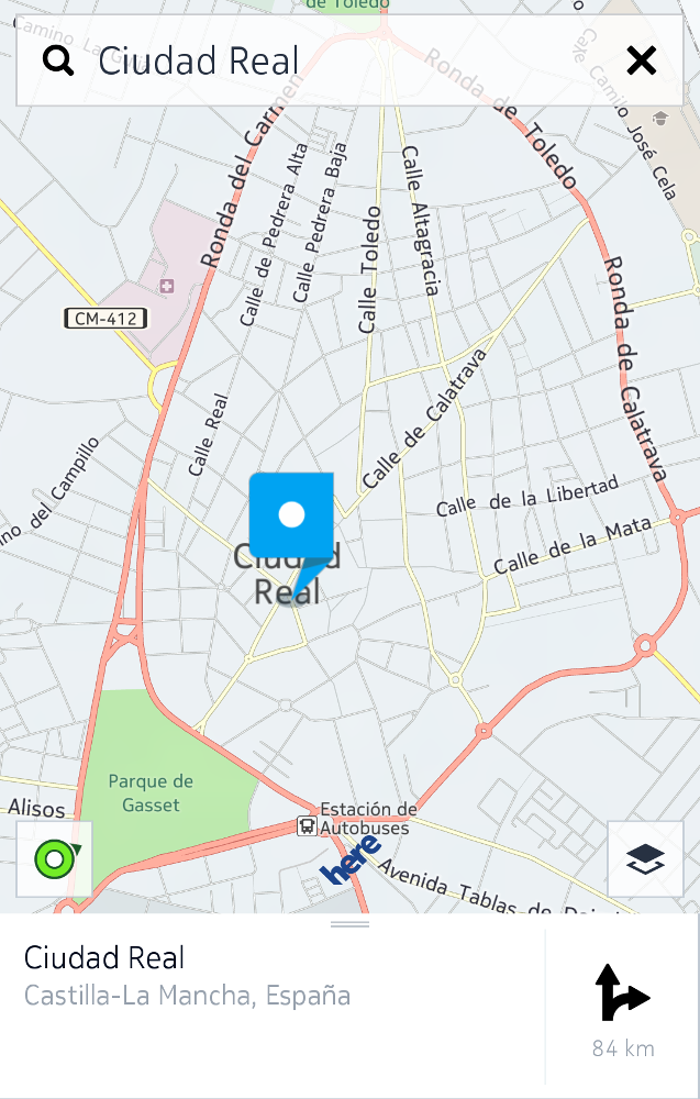
\includegraphics[height=0.6\textheight]{img/heremaps.png}
        \end{figure}
        Nokia HERE
      \end{center}
    \end{minipage}
  \end{center}
  \end{block}
\end{slide}

\begin{slide}
  \begin{block}{\textbf{Interacciones}}
    \begin{itemize}
      \item Visual, por pantalla
      \item Sonido, locuciones verbales
    \end{itemize}
  \end{block}
  \begin{block}{\textbf{Problemática}}<2>
    \begin{itemize}
      \item Mirar la pantalla = 390,000 accidentes anuales
      \item Usar cascos o auriculares = sanción de 200\EUR{}
    \end{itemize}
  \end{block}
\end{slide}

\begin{slide}
  \begin{block}{\textbf{Interacción implícita}}
    \begin{itemize}
      \item Sonido
      \item Vibración
    \end{itemize}
  \end{block}
  \begin{figure}[!h]
    \begin{center}
      \includegraphics<2>[height=0.6\textheight]{img/resumen.png}
    \end{center}
  \end{figure}
\end{slide}

% Local Variables:
%  TeX-master: "main.tex"
%  coding: utf-8
%  mode: latex
%  mode: flyspell
%  ispell-local-dictionary: "castellano8"
% End:
